%%% template.tex
%%%
%%% This LaTeX source document can be used as the basis for your technical
%%% paper or abstract.

%%% The parameter to the ``documentclass'' command is very important.
%%% - use ``review'' for content submitted for review.
%%% - use ``preprint'' for accepted content you are making available.
%%% - use ``tog'' for technical papers accepted to the TOG journal and
%%%   for presentation at the SIGGRAPH or SIGGRAPH Asia conference.
%%% - use ``conference'' for final content accepted to a sponsored event
%%%   (hint: If you don't know, you should use ``conference.'')

\documentclass[tog]{acmsiggraph}
\usepackage[T1]{fontenc}
\usepackage[utf8]{inputenc}
\usepackage[swedish, english]{babel}

%%% Make the ``BibTeX'' word pretty...

\def\BibTeX{{\rm B\kern-.05em{\sc i\kern-.025em b}\kern-.08em
    T\kern-.1667em\lower.7ex\hbox{E}\kern-.125emX}}

%%% Used by the ``review'' variation; the online ID will be printed on 
%%% every page of the content.

\TOGonlineid{45678}

%%% Used by the ``preprint'' variation.

\TOGvolume{0}
\TOGnumber{0}

\title{Perceived Depth Perception In A Virtual Environment Using A Head Mounted Display}

\author{Jesper Blidkvist\thanks{e-mail:Jesper.Blidkvist@live.se}\\Student, BTH}
\pdfauthor{Jesper Blidkvist}

\keywords{Virtual Reality, 3D, Depth Perception}

\begin{document}

%%% This is the ``teaser'' command, which puts an figure, centered, below 
%%% the title and author information, and above the body of the content.

 \teaser{
   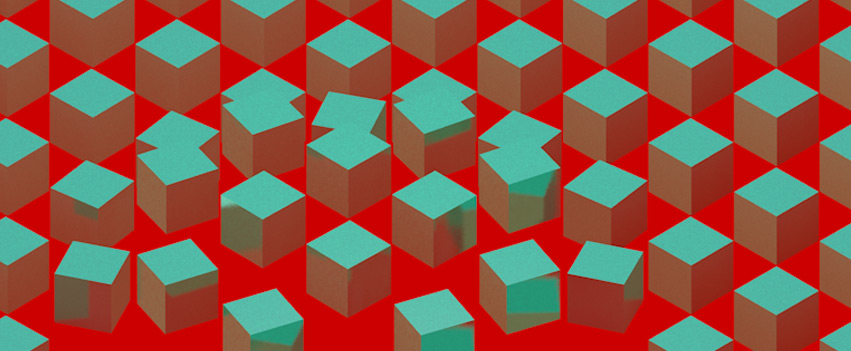
\includegraphics[height=1.5in]{images/temp}
   \caption{BTH 2015, Karlskrona, SE.}
 }

\maketitle

\begin{abstract}
In order to better understand how binocular depth cues can be recreated in a virtual environment, specifically the method of rendering a scene from two slightly differently positioned cameras, a small scale experiment was set up in which test subjects where presented with a scene containing a series of cubes and asked to estimate their distance. During the experiment the distance between the virtual cameras was either increased or decreased and the user was then again asked to estimate the distance to the cubes. While the test group was small, there where some indications that a wider distance between the cameras led to the user perceiving the cubes as being closer, and a decrease in the distance between the cameras to the user perceiving the cubes as being further away.



\end{abstract}

\begin{CRcatlist}
  \CRcat{I.3.3}{Computer Graphics}{Three-Dimensional Graphics and Realism}{Virtual Reality}
  \CRcat{H.5.1}{Information Interfaces and Presentation}{Artificial, augmented, and virtual realities};
\end{CRcatlist}

\keywordlist


\copyrightspace

\section{INTRODUCTION}

The purpose of this paper is to investigate how humans perceive depth in a virtual 3D enviroment, more specifically how the distance between the two virtual cameras can influence the users perception of depth. On a pragmatic level, this could be applied to help alleviate the scale issues experienced by some users, where objects appear too small. The ability to manipulate the users perception without changing the actual geometry of a scene could also be used for example in a multiplayer horror game, where the player upon observing something scary gets a slight increase in the distance between their virtual cameras, causing the entire scene to feel smaller without effecting actual gameplay or the scene for any other player.    

There have been a lot of research conducted in regards to human depth perception. There are also a lot of practical examples on how to manipulate our depth perception that can be found for example in art. However, with virtual reality HMDs we are offered an unique opportunity to manipulate a persons depth perception by moving the position of the virtual eyes in such a way that the depth changes. This might have been possible before, using a complicated setup of a number of mirrors but with the HMD the set up of the experiment becomes trivial.  


\begin{itemize}
\item title, author, and affiliation information
\item abstract
\item CR categories *
\item keywords *
\item body of the content
\item bibliography
\end{itemize}



\section{BACKGROUND}

In order for an observer to perceive an object and ascertain its position relative to the observers own, the brain interprets multiple sources of information, commonly referred to as cues. 
%%¤ GIBBSSSOONN!!!!(Gibson, 1950). 
These can be divided into two subcategories, binocular and monocular cues. The binocular cues works best when the distance to an object is fairly small, within 30 m ~\cite {Palvqvist:2013:DPDS}.

To perceive depth at longer distances monocular cues take precedent. While not strictly relevant to an experiment focusing on binocular depth cues, it is important to know of them since these are harder to switch of. The monocular cues are often said to to be (1) differences in shadows and light on an object (2) an object occluding or in other ways hiding one another (3) relative size of similar objects on different distances and so on. (5) the eyes lens level of accommodation, (6) loss of detail with increased distance (8) motion perspective or motion parallax.
%%%/(Kemeny &
Panerai).

The brain takes advantage of the physiological state of the eyes being approximately six inches
apart on the human head, which serves as the basis for most binocular cues. For example, this
causes the observation of a nearby object to be projected with two slightly different images on the retina as result of the two slightly different viewing angles. When these two images are merged in the striate cortex, the brain interprets the discrepancy (the binocular disparity) of the two images as a cue for depth. Thus two objects at different distances from the observer will have different amounts of such binocular disparity that signals their different locations in depth 
%%/cite Gibson. 
Ocular convergence is another binocular cue of depth. The binocular disparity in stereopsis, only works on objects that are relatively close to the observer,
approximately within 30 
%%%m /cite{Cutting & Vishton, 1995}. In



\section{EXPERIMENT SETUP}

The experiment was created using the Unity Game Engine developed by Unity Technologies an Oculus Rift HMD and a minimal amount of C\# code to allow the experimenter to change the distance between the virtual cameras at their digression. Unity was chosen as it allows for a quick experiment set up and Oculus intigration without having to create an entirely new engine.
At the time of writing there are a number of HMDs avaliable to developer, however, the Oculus was chosen for its native support in Unity and that it might be one of the most widely used HMDS.

The user is seated on a chair and places the HMD on their head. The user is then presented with a scene containing a number of cubes placed at random distances but no closer to the test subject then 3 units, and no further away then 100 units. The test subject will then be asked to look at the cubes for about thirty seconds before the screen goes black. The distance between the cameras will then be increased, and the test subject will again be presented with the scene and asked to observe for 30 seconds and then asked if anything has changed from the previous scene.  

\section{RESULT}

The title, author, and affiliation information should be centred
above the body of your content. The title should be set in a 14-point
bold sans-serif typeface with 18-point line spacing. The author and
affiliation information should be set in a 10-point serif typeface
with 12-point line spacing.

The title should be appropriately capitalized. ``All caps'' is not
appropriate. The following link provides assistance with appropriate
capitalization:

{\small\url{http://www.grammarbook.com/punctuation/capital.asp}}

Affiliations should include your educational institution or employer's
name, and a valid e-mail address.

\section{FUTURE WORK}

This experiment focused on only one depth cue. 




\section{Contact Information}

If you have questions or suggestions regarding this document, please
contact Jesper Blidkvist at ``Jesper.Blidkvist@live.se''.

\section*{Acknowledgements}

Tack till inte en jävel

\bibliographystyle{acmsiggraph}
\nocite{*}
\bibliography{template}
\end{document}
